% Filename: try31.tex
% This code is part of 'Cursos CAMECC: Introducao ao LaTeX para o Curso 29 - Licenciatura em Matematica'
% 
% Description: This file correspond exercise 31 of the textbook using in the course.
% 
% Created: 07.06.12 11:30:10 AM
% Last Change: 07.06.12 11:30:30 AM
% 
% Authors:
% - Raniere Silva, r.gaia.cs@gmail.com
% 
% Organization: CAMECC - Centro Academico dos Estudantes do IMECC
% 
% Copyright (c) 2012, Raniere Silva. All rights reserved.
% 
% This work is licensed under the Creative Commons Attribution-ShareAlike 3.0 Unported License. To view a copy of this license, visit http://creativecommons.org/licenses/by-sa/3.0/ or send a letter to Creative Commons, 444 Castro Street, Suite 900, Mountain View, California, 94041, USA.
%
% This work is distributed in the hope that it will be useful, but WITHOUT ANY WARRANTY; without even the implied warranty of MERCHANTABILITY or FITNESS FOR A PARTICULAR PURPOSE.
%
\documentclass[12pt, a4paper]{article}
\usepackage[utf8]{inputenc}
\usepackage[T1]{fontenc} 
\usepackage[top=3cm,left=2cm,right=2cm,bottom=3cm]{geometry}
\usepackage[brazil]{babel}
\usepackage{amsmath}
\usepackage{amsfonts}
\usepackage{graphicx}
\usepackage{url}

\begin{document}
\section{A função polinomial}\nocite{polinomio}
Um polinômio (função polinomial) com coeficientes reais na variável $x$ é uma função matemática $f : \mathbb{R} \rightarrow \mathbb{R}$ definida por:
\begin{align*}
p(x) &= a_0 + a_1 x + a_2 x^2 + a_3 x^3 + \ldots + a_n x^n,
\end{align*}
onde $a_0, a_1, a_2, \ldots, a_n$ são números reais, denominados coeficientes do polinômio. O coeficiente $a_0$ é o termo constante.

Se os coeficientes são números inteiros, o polinômio é denominado polinômio inteiro em $x$.
%
%Uma das funções polinomiais mais importantes é $f : \mathbb{R} \rightarrow \mathbb{R}$ definida por:
%\begin{align*}
%f(x) &= a x^2 + b x + c.
%\end{align*}

O valor numérico de um polinômio $p = p(x)$ em $x = a$ é obtido pela substituição de $x$ pelo número $a$, para obter $p(a)$.

\textbf{Exemplo:} O valor numérico de $p(x) = 2x^2 + 7x - 12$ para $x=3$ é dado por:
\begin{align*}
p(3) &= 2 \cdot (3)^2 + 7 \cdot 3 - 12 \\
&= 2 \cdot 9 + 21 - 12 \\
&= 18 + 9 \\
&= 27.
\end{align*}

\section{Sistemas de equações lineares}\nocite{sistema}
Um sistema de equações lineares ou sistema linear é um conjunto formado por duas ou mais equações lineares. Um sistema linear pode ser representado na forma:
\begin{align}
\begin{cases}
a_{11} x_1 + a_{12} x_2 + \ldots + a_{1n} x_n = b_1 \\
a_{21} x_1 + a_{22} x_2 + \ldots + a_{2n} x_n = b_ 2 \\
\vdots \\
a_{m1} x_1 + a_{m2} x_2 + \ldots + a_{mn} x_n = b_n
\end{cases} \label{eq:sis}
\end{align}
onde $x_1, x_2, \ldots, x_n$ são as incógnitas, $a_{11}, a_{12}, \ldots, a_{mn}$ são os coeficientes e $b_1, b_2, \ldots, b_m$ são os termos independentes.

Uma sequência de números $(r_1, r_2, \ldots, r_n)$ é solução de \eqref{eq:sis} se satisfaz identicamente a todas as equações desse sistema linear.

\section{Trigonometria no triângulo retângulo}\nocite{trigonometria}
Um triângulo é uma figura geométrica plana, constituída por três lados e três ângulos internos. Esses ângulos, tradicionalmente, são medidos numa unidade de medida, denominada grau e, cada um deles tem medida entre $0^o$ e $180^o$, de modo que, em qualquer triângulo, a soma dessas medidas é $180^o$.

Num triângulo retângulo definimos as chamadas razões trigonométricas que são relações entre os lados do triângulo e que têm a propriedade de determinar a medida dos ângulos do triângulo, uma vez que seus lados sejam conhecidos.
\begin{center}
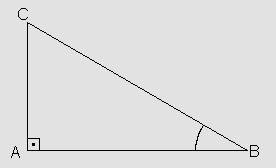
\includegraphics{triang.png}
\end{center}

No triângulo retângulo $ABC$, consideremos, por exemplo, o ângulo que tem vértice em $B$, cuja medida $\alpha$, em graus, é um número real que está no intervalo $0, \pi/2$. Entre os lados do triângulo podemos estabelecer as seguintes razões:
\begin{description}
\item[seno] é a razão entre o comprimento do cateto oposto ao ângulo $\hat{B}$ e o comprimento da hipotenusa do triângulo. Indicando o seno de $\alpha$ por $\sin(\alpha)$, temos $\sin(\alpha) = \overline{AB} / \overline{BC}$.
\item[cosseno] é a razão entre o comprimento do cateto adjacente ao ângulo e o comprimento da hipotenusa do triângulo. Indicando o cosseno de $\alpha$ por $\cos(\alpha)$, temos $\cos(\alpha) = \overline{AB} / \overline{BC}$.
\item[tangente] é a razão entre os comprimentos do cateto oposto e do cateto adjacente ao ângulo $\hat{B}$. Indicando a tangente de $\alpha$ por $\tan(\alpha)$, temos $\tan(\alpha) = \overline{AC} / \overline{AB}$.
\end{description}

\bibliography{try31}
\bibliographystyle{plain}
\end{document}
